\documentclass[12pt, a4paper]{article}
\usepackage{verbatim}
\usepackage{subfig}
\usepackage{wrapfig}
\usepackage{listings}
\usepackage{array}
\usepackage[utf8]{inputenc}
\setlength {\marginparwidth }{2cm}
\usepackage{todonotes}
\usepackage{newtxtext}
\usepackage{blindtext}
\usepackage{enumitem}
\usepackage{graphicx}
\usepackage{outlines}
\usepackage[export]{adjustbox}
\usepackage{pdflscape} % For landscape pages
\usepackage{float}     % For ordering images and text accordingly
\usepackage[colorlinks = true, urlcolor  = blue]{hyperref}
\graphicspath{ {./images/} }
\usepackage{biblatex}
\addbibresource{bibliography.bib}
\usepackage[table]{xcolor} % Add to preamble

\usepackage{hyperref}
\hypersetup{
    colorlinks=false, % Set to false if you don't want colored links
    linkcolor=blue,   % Color of links to internal documents
    filecolor=magenta, % Color of file links
    urlcolor=cyan     % Color of external links
}

\setlist[itemize]{itemsep=2pt, parsep=0pt}
\setlength{\arrayrulewidth}{0.3mm}
\setlength{\tabcolsep}{10pt}
\renewcommand{\arraystretch}{1.5}

\usepackage{xcolor}
\definecolor{light-gray}{gray}{0.95}
\newcommand{\code}[1]{\colorbox{light-gray}{\texttt{#1}}} % Functions to create code snippets with \code{code}

%\setcounter{secnumdepth}{2}

\begin{document}
\begin{titlepage}
    \centering
    \vspace*{1cm}
    
    {\Huge\bfseries DevOps, Software Evolution and Software Maintenance \par}
    \vspace{1.5cm}

    {\LARGE Group D \par}
    \vspace{1cm}
    
    {\Large Group Members: \par}
    \vspace{0.5cm}
    \begin{tabular}{rl}
        Victor Memborg-Heinrichsen & \href{mailto:vmem@itu.dk}{vmem@itu.dk} \\
        Peter Bjørholm Hansen & \href{mailto:pebj@itu.dk}{pbjh@itu.dk} \\
        Lukas Vranic & \href{mailto:luvr@itu.dk}{luvr@itu.dk} \\
        Anne-Marie Rommerdahl & \href{mailto:annro@itu.dk}{annro@itu.dk} \\
    \end{tabular}
    \vfill
    
    {\large BSc Software Development \par}
    \vspace{0.2cm}
    {\large IT University of Copenhagen \par}
    \vspace{0.2cm}
    {\large BSDSESM1KU \par}
    \vspace{0.2cm}
    {\large \today\par}
    
\end{titlepage}


\pagenumbering{arabic}
\setcounter{secnumdepth}{2}
\setcounter{tocdepth}{2}
\tableofcontents
\newpage
\section{System's perspective}
Our MiniTwit is an 'X' (formerly known as Twitter) clone written in Golang using the Gorilla web framework. It is a project that continues development on the ITU-MiniTwit system presented in the course DevOps, and it consists of a web service and an API service. 

\subsection{Architecture of MiniTwit}
MiniTwit follows the server-client architecture, and the server is deployed via a Docker Swarm, which consists of virtual machines (aka 'droplets') on DigitalOcean. Data, such as user-data, messages and followers are stored in a PostgreSQL database, which is also hosted on DigitalOcean. \\
In the swarm, we have manager-nodes and worker-nodes. The only services allowed to run on the managers are Prometheus and Dozzle (more about the swarm services in section 4). Figure \ref{fig:DeployDiagram} is a Specification Level Deployment Diagram, which shows how ITU-MiniTwit is deployed on a worker-node.
\begin{figure}[h]
\centering
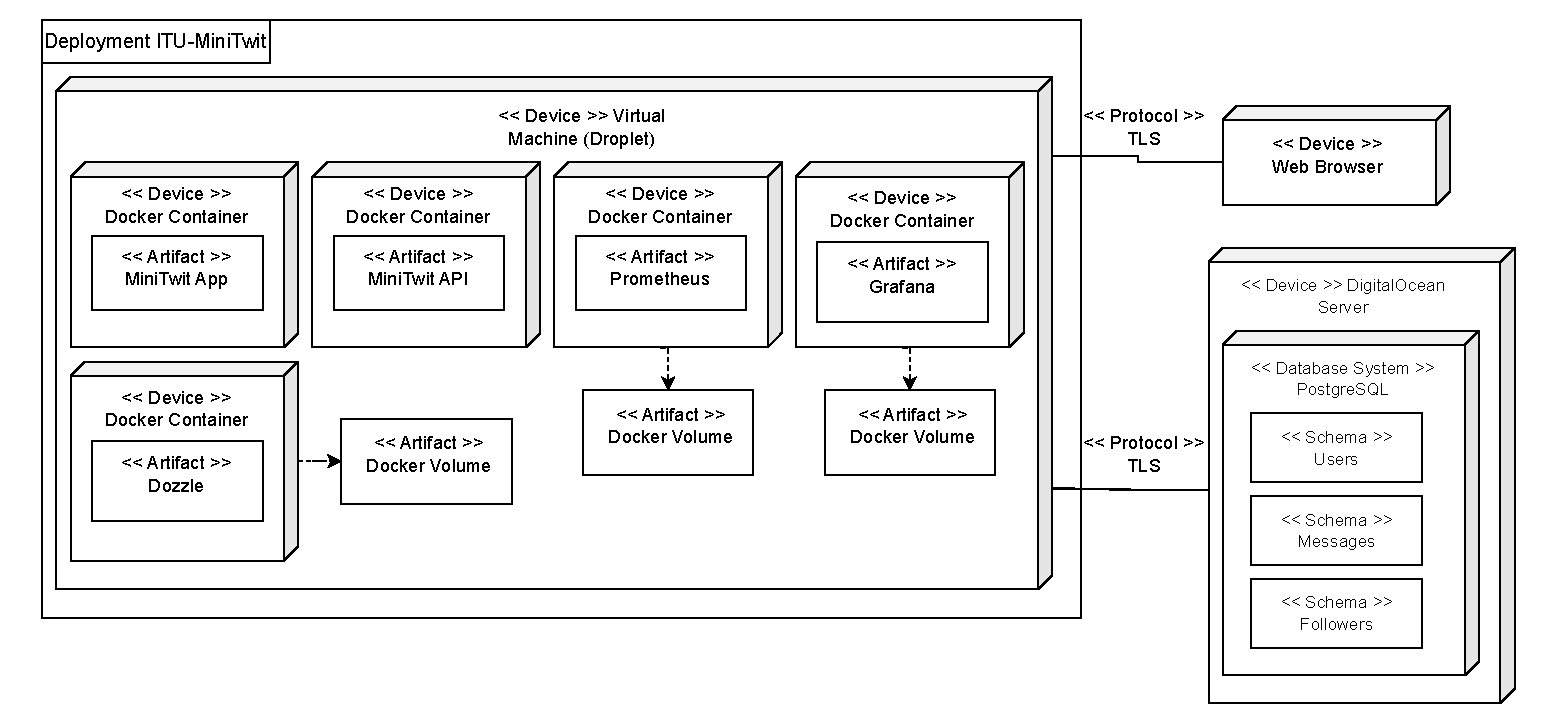
\includegraphics[scale=0.8, center]{images/DeployUMLDraft(1).pdf}
\caption{Deployment Diagram of MiniTwit on a worker node}
\label{fig:DeployDiagram}
\end{figure}

\subsection{Dependencies of MiniTwit}
This project relies on several dependencies across different project areas, including runtime, testing, and infrastructure. The dependencies have been kept up-to-date using Dependabot.

\subsubsection{App and API}
Our app and API are built in Go 1.23.0, and rely on the following direct dependencies:
\begin{itemize}
    \item \textbf{github.com/gorilla/mux:} Router for HTTP request routing.
    \item \textbf{github.com/gorilla/sessions:} Session management for user authentication.
    \item \textbf{gorm.io/gorm} and \textbf{gorm.io/driver/postgres:} GORM ORM and PostgreSQL driver for database operations.
    \item \textbf{github.com/prometheus/client\_golang:} Exposes Prometheus metrics endpoints for monitoring.
\end{itemize}

\subsubsection{Testing}
\begin{itemize}
    \item \textbf{Go:}
    \begin{itemize}
        \item \textbf{Go's built-in testing package:} Go's native testing framework
        \item \textbf{Testify:} Used for more assertions and mocking
        \item \textbf{github.com/mattn/go-sqlite3:} Creates a local testing database
    \end{itemize}

\item \textbf{Python:}
\begin{itemize}
    \item \textbf{Pytest:} Testing framework
    \item \textbf{Selenium:} Browser automation for UI testing
    \item \textbf{Requests:} HTTP client library for API testing
\end{itemize}
\end{itemize}

\subsubsection{Infrastructure}
\begin{itemize}
    \item \textbf{Docker:} Used for containerizing both the API and the app. Docker compose was used during development to orchestrate services. Later in the project, Docker Swarm was adopted to deploy containers across multiple nodes in production.
    \item \textbf{Virtual Machines:} The swarm nodes are hosted on VMs (DigitalOcean Droplets in this project).
    \item \textbf{Docker Hub:} Used to distribute container images. The CI/CD pipeline pushes API and app images to Docker Hub for swarm nodes to pull.
    \item \textbf{PostgreSQL:} Main production database, managed as a hosted database in Digital Ocean.
    \item \textbf{Prometheus:} Scrapes and stores metrics from both the app and API and from itself.
    \item \textbf{Grafana:} Visualizes metrics collected by Prometheus.
    \item \textbf{Dozzle:} Provides a real-time web UI for viewing container logs in Docker Swarm.
\end{itemize}

\subsection{Interactions of subsystems}

Depending on which kind of request sendt to MiniTwit. It will either be handled by the app or API. They both use the same database, so the data will be shared between them both. The sequence diagrams below, how they handle a post message request. Figure \ref{fig:user-seq} shows how a user request is handled and figure \ref{fig:api-seq} shows the same for the api.

\begin{figure}[H]
% https://editor.plantuml.com/uml/RLDTRzem57tthpZAmmGITKkxpqYRMifA9ws3alHX4X8oyHru2p7oHrbLxR_F9aaBLPyYNvzpxZt7D-VM2UFykcIYSDhWpf9Xcr1IXTg8oc5WzFPbBHbfP6JkoSogpeMKDsIjMDArg6H9ffj0sER-a9O5dD8Lij290dMaZIfBWQPkM-RkzABZU7eJ61DjtT9GTlkzniRo8V0PiGCC1un5JpZwqbf9qUV8_6AjdCMw7Xs_j5b7_N6MurX8EMykkgnXHO7QKufJZkiydo2Y0-agS5Cu-kjwkDJwZw8KjZRHPQmcrVHTBSKPR-zxc2Fz3EzKQVc8N0Ffc1wsNTRcTRJN-orlTI254-ZuCDnSoODECPOKxpWk3Gb7dJUjcrcLEUCBb-BnmhkLZimUyZZwh9hunJneKWzNfLWkIVvZKIWA3WSftdDy-v5zdURXau_Rv6m8W7FUPSF1RiwwzGUEMq_c0TONHG0sGdi-Fd9CoVhIGIz-K-5U3UeJRw89InPcigjES93yrDuyFTmsFBAXGXj9CdariVu9nuxynB5n_-H-n-VLw3TlUtPo6WQKAcWxE8taEDbVXRiQ7JOXM-aj_2O69-7KcafL4MFdLCdmM_q7
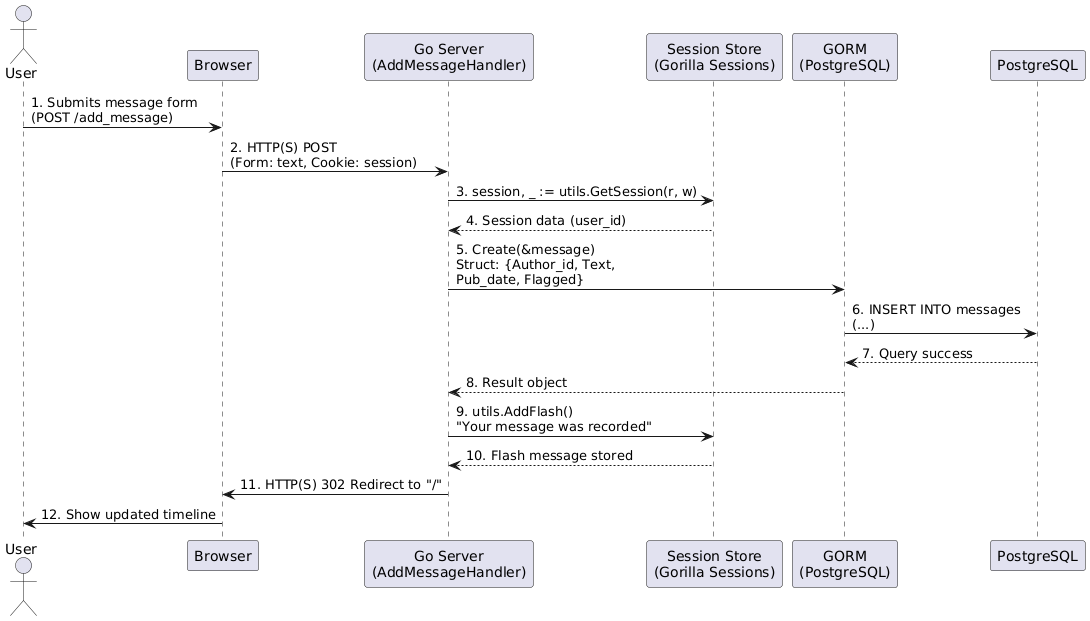
\includegraphics[width=\textwidth]{images/user-seq-diagram.png}
\centering
\caption{Sequence diagram of a user posting a messages.}
\label{fig:user-seq}
\end{figure}
% https://editor.plantuml.com/uml/TLJRJjj047tVhnZvYKXWI4XRy4DBIfkKYbp0KAegKhJnJfDLxTsmkuQuY7_l-59ifzIIR-CpPywS6VdCEcvSciJCIHSZ36ON0HmcTcKFdrABHl44d-6p4XijbOCGxrDK4J8UEMt08pYSnnALcwkzK2Pfp2dUyO3RAiusn2yZkU6KxeqqKPW7D0MYV6mZnbA861-vmG9IlxPXNxYYk9ch1AtbAxGpDBUsugq-xfIUNez9v4nRjp8ONbsMAlDm6pYKv4EOMOT9WHY6Z9MzmC7xIdC0NHzcq_3c7w_cQf2wTG0VkPKHHBtOYRljMenEiwcQTAFHj-pxyMJz8xbTiv8g9wsx3A3dGxeHtE4bdTRjcGwhF-VWOHZ0iGztHZg4k00jDaP7P0IAXPN9WeOZjLf8uRkjOyCG3dPgzF-cspJAyreL6as-yU5SAoTLYb2La6h56iehgmDuIz0rHh-0K_lQoDyyrq26A-skyNveT5Bl1wlIMiNU-J1evi83ZwLWDRPHhKlAFc6a1SBNS3g1fHRPN3rv4QcbGNa1UDLYWCEjyvwRBFd8YO8KNwLeCiXd1ylodi-GvO12MbsFnENh1TGD_DIf4XyOZzrEZ04TpTRAjQ7q4-v3_wXFijeP7iFOOadp2iMBrfCbsMkGXWqA7s5SzaRkbexHgFVXXXhTXrcwNEJRqocONkdar8SBHVNSo_3_fxftvDD9eYSQAcCPaaHsHbVwPVm1
\begin{figure}[H]
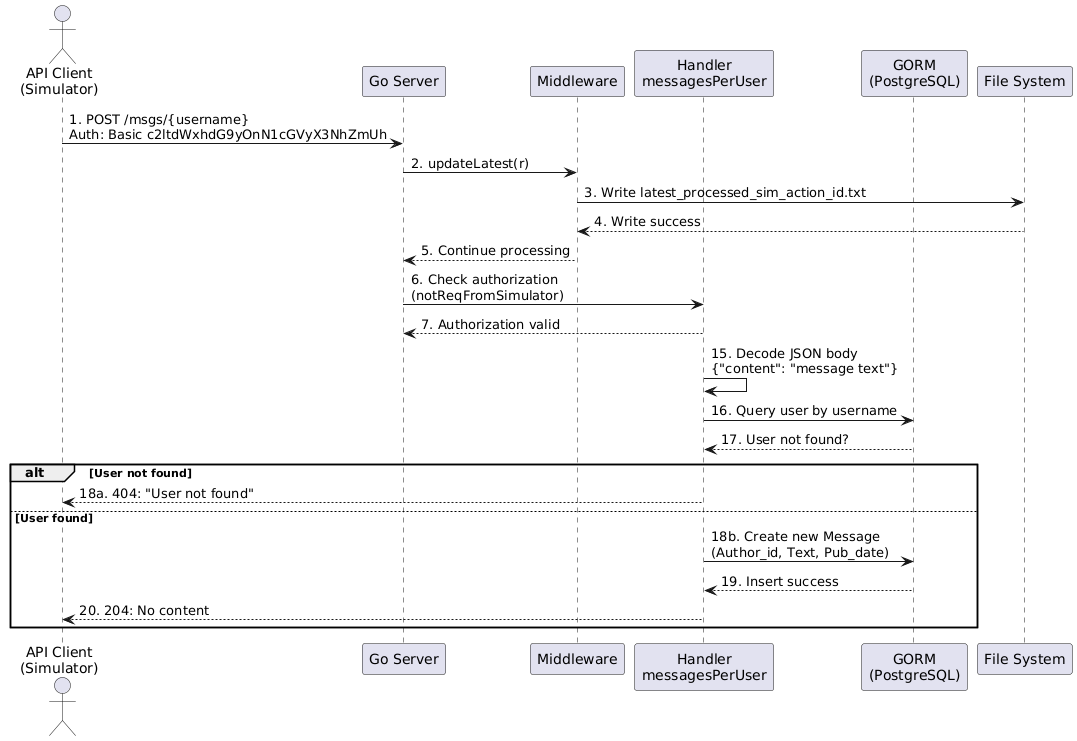
\includegraphics[width=\textwidth]{images/api-seq-diagram.png}
\centering
\caption{Sequence diagram of a api posting a messages.}
\label{fig:api-seq}
\end{figure}


\subsection{Current state of MiniTwit}
We have implemented the two tools Sonarqube and Code Climate, which can assist in estimating the maintainability and technical debt of our project.
\subsubsection{Code Climate}
Code Climate reports 10 code smells, 0 duplications and 0 other issues. This leaves us with an A-rank (see figure \ref{fig:CodeClimate})\\
\begin{figure}[h]
\centering
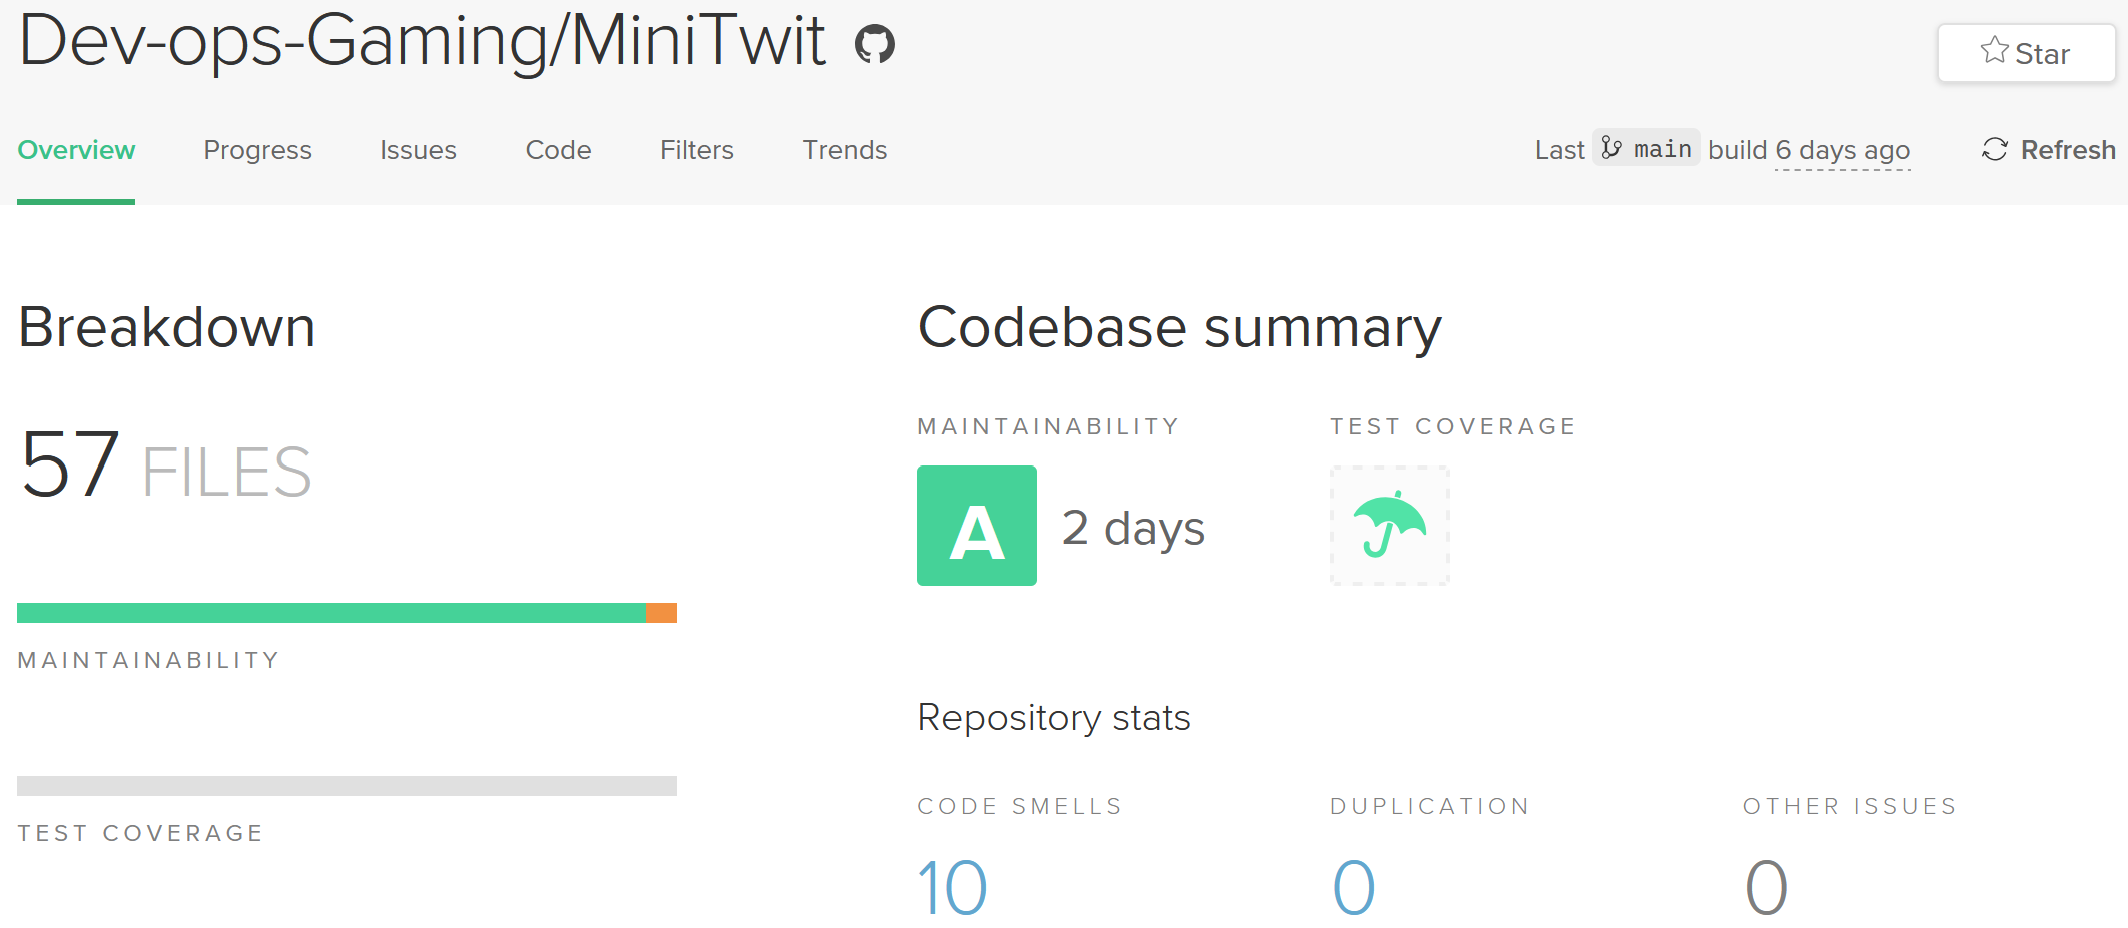
\includegraphics[width=\textwidth]{images/code_climate.png}
\caption{Overview of MiniTwit on Code Climate}
\label{fig:CodeClimate}
\end{figure}

\subsubsection{Sonarqube}
Sonarqube reports 18 issues - all in the category 'maintainability' - and 0.9\% code duplication (see figure \ref{fig:SonarQube}). A majority of these issues are found in the tests, and many of the issues are in regards to string duplicates.
\begin{figure}[h]
\centering
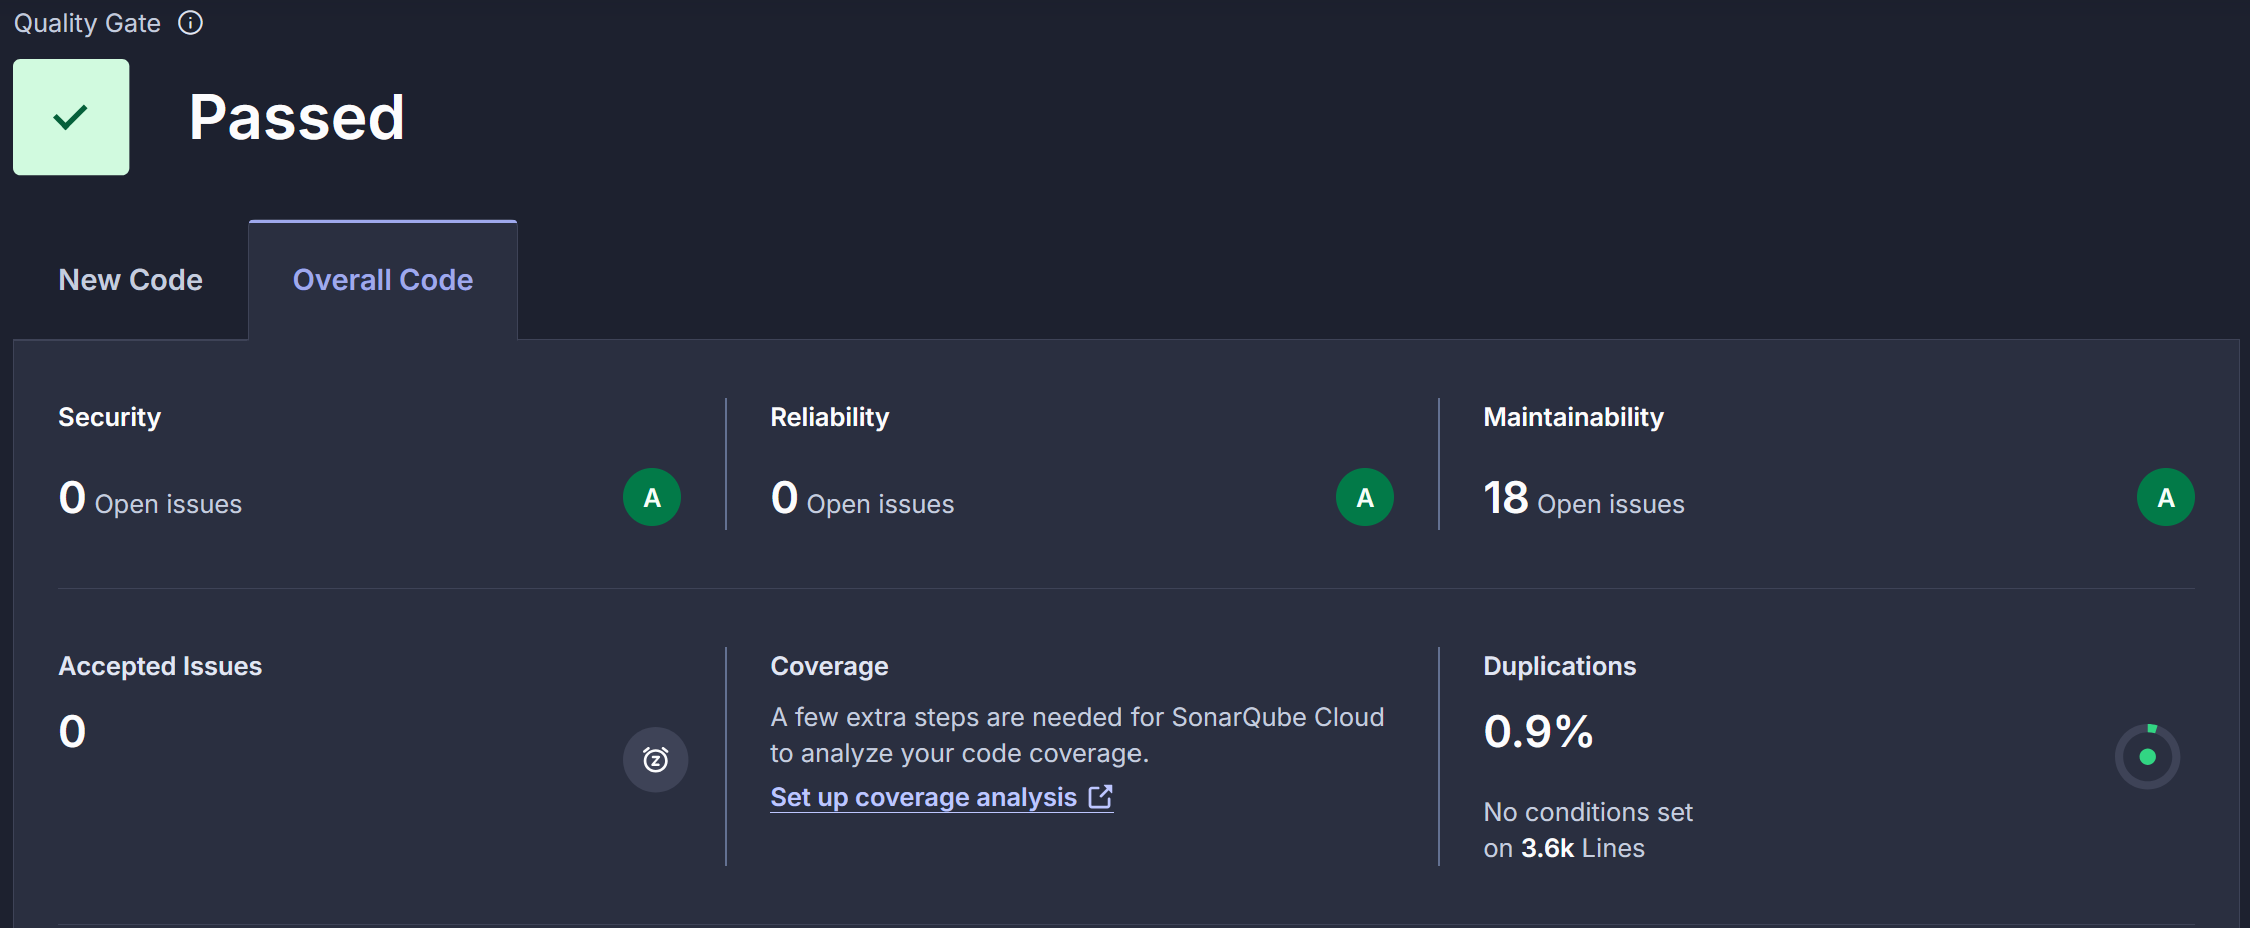
\includegraphics[width=\textwidth]{images/sonarQube.png}
\caption{FIX POSITION OF THIS WHEN REPORT ALMOST DONE!! Overview of MiniTwit on SonarQube}
\label{fig:SonarQube}
\end{figure}
\section{Process' perspective}
\subsection{Security Assessment}
To protect our system against adversaries, we first identify the assets that must be protected. We then identify which threats we could face and how. Finally, we analyze these scenarios to figure out which scenarios pose the biggest threats.

\subsubsection{Risk Identification}
Our assets:
\begin{itemize}
    \item Codebase
    \item Database
    \item Logs
\end{itemize}

Threat Sources:
\begin{itemize}
    \item SQL Injection
    \item Exposed ports (Prometheus)
    \item Vulnerable password hashing
    \item No requirements for user password (length, symbols, etc.)
    \item Vulnerable dependencies
    \item No password on Dozzle (logging)
\end{itemize}

Risk Scenarios:
\begin{itemize}
    \item A - Attacker performs SQL injection to download sensitive user data
    \item B - Attacker performs SQL injection to delete information from the database
    \item C - Attacker performs SQL injection to log in to a legitimate user's account
    \item D - Attacker brute-forces the hash of a password, letting them log in to a legitimate user's account
    \item E - Attacker uses the open ports to overload our Prometheus with queries
    \item F - Attacker intersects messages sent over the network, as they are not encrypted*** (attacker reads messages, or does man-in-the-middle to send their own messages to user)
    \item G - Attacker exploits a vulnerable dependency, which lets them perform some malicious attack. As the actual threat level depends on the specific vulnerability, we've chosen to be pessimist and assume, that the consequences will be disastrous
    \item H - Attacker accesses our logs on Dozzle, which lets them see all outputs, like usernames
\end{itemize}

\subsubsection{Risk Analysis}
Here are the scenarios presented on the risk matrix:
\begin{center}
\begin{tabular}{ |c|c|c|c|c| } 
 \hline
  & Rare & Unlikely & Likely & Certain \\ 
 \hline
 Catastrophic & B &  &  & G\\ 
 \hline
 Critical & A &  &  & \\ 
 \hline
 Marginal & &  &  F& E\\ 
 \hline
 Negligible & C &  & D & H\\ 
 \hline
\end{tabular}
\end{center}
Scenarios A, B, and C have a 'Rare' probability, as we already utilize the ORM-library 'GORM'. GORM uses prepared statements and automatically escapes arguments to avoid SQL injection. Without GORM, the probability would be much higher.\\
Scenario F was dealt with using the TLS protocol. Our Minitwit application using TLS is hosted at https://lukv.dk.\\
For scenario G, we have added Dependabot, which will automatically search for outdated dependencies, and create pull requests to update such dependencies.
\\\\
\\
For scenario E, we would have to perform a workaround, as the exposed ports are caused by Docker and UFW being incompatible, an issue which has not yet been patched. However, Prometheus is the only service that is exposed, and the only threat is Prometheus crashing due to an overload of queries. Therefore, it is not considered a high-priority threat.
\\\\
\\
Scenario H can be prevented by locking our Dozzle interface with a password. However, no sensitive data is logged in Dozzle, and thus it is considered low priority.

\subsection{Scaling and Upgrades}
\subsubsection{Scaling}
To scale our Minitwit application, we performed horizontal scaling using Docker Swarm. We created three manager nodes and four worker nodes. \\
We have replicas of the following services:
\begin{center}
\begin{tabular}{ |c|c|c| } 
 \hline
 Service & Replicated/Global & No. of replicas \\ 
 \hline
 Minitwit App & Replicated & 3 \\ 
 \hline
 Minitwit API & Replicated & 4 \\
 \hline
 Prometheus & Global & N/A \\ 
 \hline
 Dozzle & Global & N/A \\ 
 \hline
\end{tabular}
\end{center}

Prometheus and Dozzle are set to be global services, meaning that one instance of each runs on every node in the swarm. This ensures that monitoring and logging are consistently performed on all nodes, preventing any loss of critical information, whether it is logging or monitoring, due to missing coverage.

\subsubsection{Upgrades}
We use a rolling update strategy with a start-first-order to update the services in our swarm. This means that one replica at a time is updated by starting a new container before stopping the old one, ensuring minimal downtime. Updates are monitored for 30 seconds, and if any failures are detected, our swarm will automatically roll back to the previous working version \cite{dockerComposeDeploy}.

\subsection{CI/CD Chain}
We are using GitHub Actions to automate the testing and deployment of Minitwit. There are 5 GitHub Actions workflows:

\begin{outline}[enumerate]
    \1 Deploy services to DigitalOcean
        \2 Runs when there is a push to \code{main}.
        \2 This workflow builds and pushes Docker images to Docker Hub, it then pulls them onto to the server on DigitalOcean.
    \1 Run tests and linter
        \2 Runs on any push or when a PR is updated/created.
        \2 Runs linters and tests on new commit or PR.
    \1 Release MiniTwit
        \2 Runs every thursday at 23:30 UTC.
        \2 Creates a weekly release of MiniTwit.
    \1 Run linter
        \2 Runs when called by other workflows.
        \2 Lints Go files using golangci-lint.
    \1 Hadolint on dockerfiles
        \2 Runs when called by other workflows.
        \2 Lints Docker files using Hadolint.
\end{outline}
\begin{figure}[H]
    \centering
    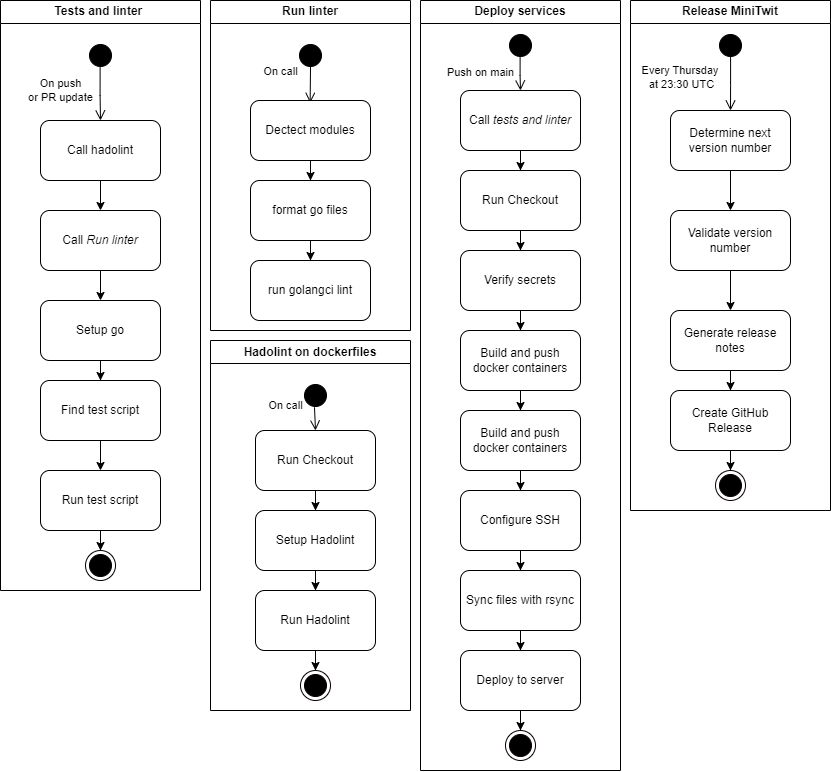
\includegraphics[width=\textwidth]{images/Worflows.png}
    \caption{Activity diagram of the workflows.}
\end{figure}


\subsection{Monitoring}
We monitored MiniTwit using Prometheus for collecting metrics and Grafana for visualizing them. This setup provided great insights into the application's performance and behavior.

\subsubsection{Prometheus}\label{prom}
Prometheus was integrated into both the API and the application through a custom middleware that intercepts HTTP requests to gather metrics. The metrics collected includes:

\begin{itemize}
\item \texttt{http\_requests\_total}: A counter that counts the total number of HTTP requests. It includes labels for request path, HTTP method, and status code. This metric helped us monitor request load per endpoint, track response statuses (in general or just on an endpoint basis).
\item \texttt{http\_request\_duration\_seconds}: A histogram measuring the time taken to process HTTP requests, in seconds. It is labeled by request path and method, enabling performance benchmarks for endpoints.
\item \texttt{http\_response\_messages\_total}: A counter that logs the total number of HTTP responses, categorized by status code and message type. Before logging was fully implemented, this metric was particularly helpful in identifying which endpoints triggered specific status messages and understanding the reasons behind them. A bit deprecated as soon as logging was implemented.
\end{itemize}

Seen in retrospect, it would have been a good idea also to collect metrics on database queries, but this will be described more thoroughly in section \ref{maintainence}

\subsubsection{Grafana}
Althoughugh Prometheus was important for collecting data, Grafana is utilizto visualize the data. Grafana connects to Prometheus as a data source, enabling the creation of dashboards. As mentioned in section \ref{prom} we monitored both our API and app, which resulted in us setting two dashboard up; one for the app and one for the API.
\\\\
For instance, the API dashboard converted the metrics collected by Prometheus into a clear visual representation of the API's health and performance. Panels were set up to showcase:
\begin{itemize}
    \item Indicators from \texttt{http\_requests\_total}, such as the rate of requests per second, overall request load distributed by endpoint, and the ratio of successful and client-error status codes.
    \item Performance monitored by \texttt{http\_request\_duration\_seconds}, including average response times and 99th percentile latency, allowing for quick identification of performance degradation.
\end{itemize}

\subsection{Logging}
Logging in MiniTwit was implemented using Dozzle. When we initially wanted to implement logging, we implemented an ELK stack in our standard Docker Compose. This was a very basic implementation with no parsing or user setup. However, this never made it to production because while it was being worked on, we implemented Docker Swarm, and suddenly, a lot changed for our system. Meanwhile, another group member noticed a TA proposing a look at Dozzle if you had problems with ELK. Dozzle was implemented with great success in no time and worked great for us.

\subsubsection*{What do we log in Minitwit?}
In Minitwit, we log application events using Go's standard logging functions, including error messages from our main application and API services. Our database layer (GORM) is configured to log at a warning level. We also log API error responses and critical application failures.

\subsubsection*{How do we aggregate logs?}
All logs in Minitwit are aggregated at a container level using Docker’s built-in logging, with every service writing to \texttt{stdout} and \texttt{stderr}. We use Dozzle, deployed in global mode in our swarm, to view and search logs from all running services in real time through its web interface. 

\subsubsection*{Why we choose Dozzle}
We ended up using Dozzle because it enabled us to filter logs by container and log level. We can transmit logs from our services in real time and filter them by service and different logging levels. A sidebar is available, which is equipped with a fuzzy search ability and provides a comprehensive overview of each service, node, replica, and swarm manager. It offers a standard search within the logs for manual searches and the ability to conduct Regex searches within the logs. Dozzle is a simple and effective method of logging, as it is not infrastructure-intensive and is extremely lightweight. Implementation within a Docker swarm is effortless with Dozzle. Dozzle was the optimal choice for us due to its user-friendly interface and all of the aforementioned.

\subsubsection*{ELK stack features we missed out on}
We cannot implement a role-based access control or authentication system with Dozzle, which is unsuitable for production. As of now, unauthorized users can see our logs, and that is, as mentioned, potentially a security breach. We cannot save our logs indefinitely, and cannot distinguish between what should be parsed and what should not. Additionally, we are forfeiting the performance that Elasticsearch would have offered through its robust indexing and search capabilities.
\\\\
While there is a lot more we miss out on not using an ELK stack, these are the ones we feel were relevant to us. An ELK stack would require much more management, and you could almost endlessly improve it. We feel that Dozzle provided us with what we needed. Combined with our monitoring, we have the opportunity as developers to quickly gain an overview of bottlenecks or bugs in the application and fix them accordingly. 
\section{Reflection Perspective}
\subsection{Evolution and Refactoring}


\subsection{Operation}\label{operation}
\subsubsection{Adding indexes}
As we monitored the performance of our API and web application throughout the project, we noticed a degradation in response times. At one point, the \texttt{/public} endpoint was particularly affected, with average response times reaching up to 70 seconds. This was unacceptable, and we began investigating the cause.
\\\\
Although we had not implemented database query monitoring through prometheus, we suspected that the bottleneck might lie in our SQL queries. Looking at the performance metrics provided by DigitalOcean, where our PostgreSQL database is hosted, we identified that the \texttt{queryMessages} method was the cause of this issue, and it became clear that we needed to index on frequently queried columns. The indexation resolved the issue, and our \texttt{/public} endpoint has since then had a response time of 20-50ms. In future projects, it will be optimal to monitor the database execution time and visualize it as a \texttt{Time series} in Grafana to see if queries degrade over time.

\subsubsection{API terminating}
The very first issue we encountered was the API becoming unavailable due to crashing when the database encountered an error. We had a hard time debugging this, as the crash did not provide any valuable information in the Docker logs (a logging tool had not been introduced yet), only to discover that we used \texttt{panic}, which causes the program to terminate in Go. This took a bit of time to realize, but when we finally traced the issue, we replaced the panic call with returning a proper status code and tried to enforce more thorough code reviews, and although implemented a bit late, we integrated our testing suite into our CI flow as shown in section \ref{cicd}.

\subsection{Maintenance}\label{maintainence}
\subsubsection{Disk usage}
One valuable lesson we have learned during the course was the importance of managing disk space in production. At one point, we lost the ability to SSH into our main droplet. We used the recovery console to investigate the issue and discovered that the disk was completely full. After analyzing the disk usage, we found that whenever we deployed a new version of minitwit, we pulled the latest image, but didn't delete the old one, which slowly consumed all the storage. To resolve this, we removed the old images, scaled the storage vertically, and have since been more observant of disk usage. Although not yet implemented, it would also be a good idea to prune old unused images automatically when pulling new ones.

\section{Usage of AI-assistants}
We utilized two large language models (LLMs) throughout the project to support our development process: GitHub Copilot and ChatGPT. GitHub Copilot was primarily used for code completion and was constantly active during development. ChatGPT, on the other hand, was used to quickly gain an overview of how to attack an issue, e.g., the database index issue described in section \ref{operation} or a tutor conveying the essential documentation for e.g., our web framework "Gorilla".
\\
We found that the LLMs significantly improved our workflow by accelerating learning and implementation. However, we suspect Copilot of introducing the API issue also described in \ref{operation}, so it is important to be critical when utilizing these tools.
\section{Artifacts}
\begin{itemize}
    \item \href{https://github.com/Dev-ops-Gaming/MiniTwit}{MiniTwit repository}
    \item \href{https://github.com/Dev-ops-Gaming/report}{Report repository}
    \item \href{https://github.com/Dev-ops-Gaming/MiniTwit/issues}{Issue tracking}
    \item \href{http://209.38.176.56:8080/}{App}
    \item \href{http://209.38.176.56:8088/}{API}
    \item \href{http://209.38.176.56:3000/}{Monitoring}
    \item \href{http://209.38.176.56:8088/}{Logging}
\end{itemize}

% Print the bibliography
\newpage
\printbibliography
% \newpage
% \input{sections/apendix}
\end{document}